\documentclass[12pt, twoside]{article}
\usepackage[letterpaper, margin=1in, headsep=0.5in]{geometry}
\usepackage[english]{babel}
\usepackage[utf8]{inputenc}
\usepackage{amsmath}
\usepackage{amsfonts}
\usepackage{amssymb}
\usepackage{tikz}

\usepackage{yhmath} %for wideparen function of over-arc
%\usetikzlibrary{quotes, angles}

\usepackage{graphicx}
\usepackage{enumitem}
\usepackage{multicol}

\usepackage{fancyhdr}
\pagestyle{fancy}
\fancyhf{}
\renewcommand{\headrulewidth}{0pt} % disable the underline of the header

\fancyhead[RE]{\thepage}
\fancyhead[RO]{\thepage \\ Name: \hspace{3cm}}
\fancyhead[L]{BECA / Dr. Huson / 10th Grade Geometry\\* 2 April 2019}

\begin{document}
\subsubsection*{9.6 Homework: Circle angles}
 \begin{enumerate}

\item Write down the formula for the circumference of a circle given the radius. \vspace{1cm}
\item Write down the formula for the area of a circle. \vspace{1cm}

\item Given circle $O$ with radius $OB=4$.
  \begin{multicols}{2}
   \raggedcolumns
   \begin{enumerate}
     \item Find the circumference of circle $O$. \vspace{1.7cm}
     \item Find its area.  \vspace{2cm}
     \item Given that $m\angle AOB=60^\circ$, find $m \wideparen{AB}$. \vspace{1cm}%yhmath package
     \item Find the area of the sector $AOB$. \vspace{1.5cm}
   \end{enumerate}
     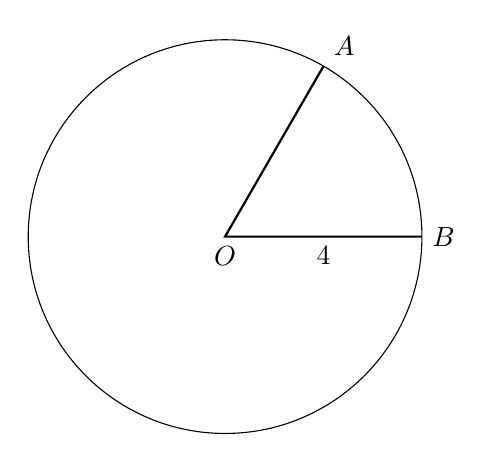
\begin{tikzpicture}[scale=.5]
       \draw (0,0) circle[radius=5];
       \draw [thick]
       (0:5) node[right] {$B$}--
       (0,0) node[below] {$O$}--
       (60:5) node[above right] {$A$};
       \draw (2.5,0) node[below] {$4$};
     \end{tikzpicture}
  \end{multicols}  \vspace{2cm}

\item Given circle $P$ with $m \wideparen{AB}=80^\circ$.
  \begin{multicols}{2}
   \raggedcolumns
   \begin{enumerate}
     \item Write down the $m\angle APB$. \vspace{1.7cm}
     \item Find the $m\angle AQB$. \vspace{2cm}
   \end{enumerate}
     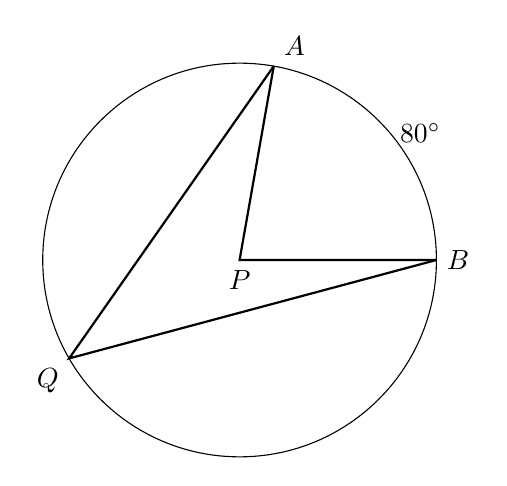
\begin{tikzpicture}[scale=.5]
       \draw (0,0) circle[radius=5];
       \draw [thick]
       (0:5) node[right] {$B$}--
       (0,0) node[below] {$P$}--
       (80:5) node[above right] {$A$};
       \draw [thick] (0:5)--(210:5) node[below left] {$Q$}--(80:5);
       \draw (40:5) node[right]{$80^\circ$};
     \end{tikzpicture}
  \end{multicols}

\newpage

\item Given circle $O$ with chords $\overline{AD}$ and $\overline{BE}$ intersecting at $C$, as shown in the diagram. Given $m \wideparen{AB}=50^\circ$, $m \wideparen{BD}=100^\circ$, and $m \wideparen{DE}=70^\circ$.
  \begin{multicols}{2}
   \raggedcolumns
   \begin{enumerate}
     \item Find the $m\angle BAD$. \vspace{1.7cm}
     \item Find the $m\angle ACB$. \vspace{2cm}
   \end{enumerate}
   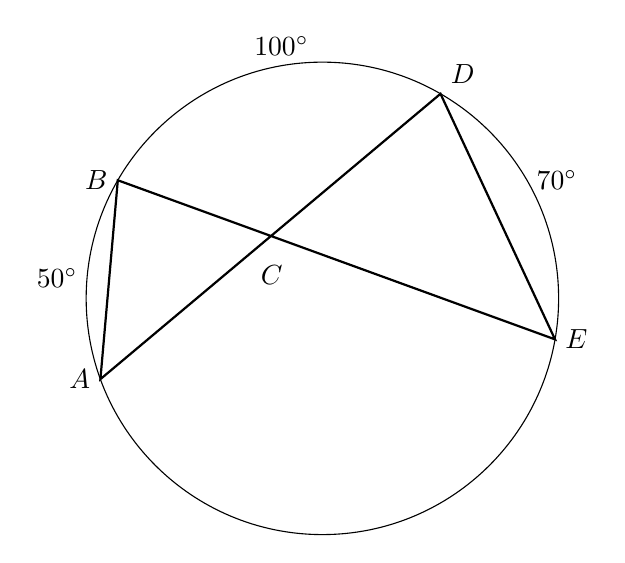
\begin{tikzpicture}[scale=.6]
     \draw (0,0) circle[radius=5];
     \draw [thick]
     (-10:5) node[right] {$E$}--
     (150:5) node[left] {$B$}--
     (200:5) node[left] {$A$}--
     (60:5) node[above right] {$D$}--cycle;
     \draw (140:1.4) node[below] {$C$};
     \draw (30:5) node[right] {$70^\circ$};
     \draw (100:5) node[above] {$100^\circ$};
     \draw (175:5) node[left] {$50^\circ$};
   \end{tikzpicture}
  \end{multicols}

\item The secants $\overline{ABC}$ and $\overline{ADE}$ intersect the circle $O$, as shown in the diagram. Given $m \wideparen{BD}=30^\circ$ and $m \wideparen{CE}=140^\circ$.
   \begin{enumerate}
       \begin{multicols}{2}
         \item Find the $m\angle CDE$.
         \item Find the $m\angle BCD$.
       \end{multicols}  \vspace{2.5cm}
     \item Find the $m\angle A$. \vspace{0.5cm}
   \end{enumerate}
     \begin{center}
     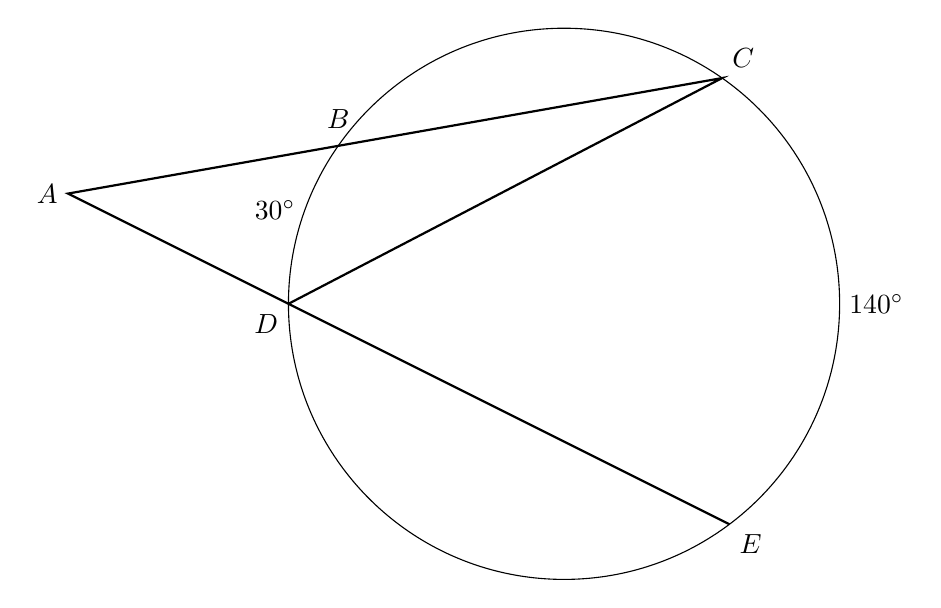
\begin{tikzpicture}[scale=.7]
       \draw (0,0) circle[radius=5];
       \draw [thick]
       (3,-4) node[below right] {$E$}--
       (-5,0) node[below left] {$D$}--
       (-9,2) node[left] {$A$}--
       (55:5) node[above right] {$C$}--
       (-5,0);
       \draw (138:5) node[left] {$B$};
       \draw (0:5) node[right] {$140^\circ$};
       \draw (160:5) node[left] {$30^\circ$};
     \end{tikzpicture}
    \end{center}


\end{enumerate}
\end{document}
